% https://www.doi2bib.org

\documentclass[twocolumn]{article}
\usepackage{geometry}
\usepackage{hyperref}
\hypersetup{
    colorlinks=true,
    linkcolor=blue,
    filecolor=blue,      
    urlcolor=blue,
    citecolor=blue,
    pdftitle={Overleaf Example},
    pdfpagemode=FullScreen,
    }
\usepackage{lipsum} % For dummy text
\usepackage{graphicx} % For including images
\usepackage{fancyhdr} % For custom headers and footers
\usepackage[style=numeric,sorting=none]{biblatex}
\addbibresource{references.bib} % Name of your bibliography file

% Set up geometry
\geometry{a4paper, margin=1in}

% Set up header and footer
\pagestyle{fancy}
\fancyhf{}
\fancyhead[L]{\textbf{NER '25 Problem Outline}}
\fancyhead[R]{\today}
\fancyfoot[C]{\thepage}

\title{NER '25 Problem Outline}
\author{Shaan, Bernardo, Alejandro, Muhammed}
\date{}

\begin{document}

% 
% also want validation of power measurements
% compare results of your power estimation of lets say fft
% to similar FPGAs or ASICs that are already out there
% don't have to completely validate it - just extrapolate to show roughly true
% 2 pipelines - 1. shiao inspired, 2. neo-inspired.

% 

\maketitle

\section{Introduction}

\begin{verbatim}
    Introduction:
    Compute on BCIs is important
    What methods fit on device?
    X tool solves this problem
    easy to integrate into existing workflows
    validated with real hardware

    Motivation:
    2 algorithms contrast them with hardware availability

    Description  of the tool:
    GUI

    Validation results

    Future work and other uses:
    FDA and others
    
\end{verbatim}


Brain-computer Interfaces (BCIs) provide opportunities to treat neurological disorders, understand brain functionalities and interface brains with the digital world. As the field of BCIs has matured, it has given rise to more complex and data-intensive models that require efficient, real-time processing to be effective. These models can no longer rely on generic processors to meet their bespoke computational demands; instead, they require the design of custom hardware to support their models.

Neuroengineers commonly use software simulations to prototype and evaluate novel algorithms for BCIs. However, neuroengineers are not usually experts in hardware design and so often can't make the best choices for their use cases. This leaves a lot of performance and potential errors in their algorithms, originally designed at the software level yet implemented at the hardware level. Furthermore, today there is no clear consensus on what constitutes an optimal BCI algorithm, such as for seizure prediction, with many different ideas present and no clear way of comparing them.

All these issues necessitate a development and evaluation platform for BCIs -- one that allows neuroengineers to prototype and evaluate hardware-level BCI algorithms without being expert hardware engineers.

\section{Significance}

The field of BCIs is growing at a rapid rate, with increasingly larger and a wider variety of computation models such as SCALO \cite{10.1145/3579371.3589107}. However, there is no standardised method for prototyping and evaluating these models, leading to an increased workload for neuroengineers to test their ideas, particularly in the case of creating hardware based tests. There is a need for a standard method of developing complex hardware based BCI systems that will lead to greater productivity and product quality. Furthermore, ensuring the quality of BCI software is crucial for its acceptance and integration by a wider audience. A well-designed and tested pipeline increases trust and confidence in the technology, leading to broader adoption.


\section{Similar work}

There is a large variety of BCI simulators available in literature, however, they are mostly non-modular and none support hardware-level simulation of BCI algorithms. Furthermore, they are generally crafted towards the use of non-invasive BCIs and EEG signals, although it can be seen how they could be modified with a little bit of work to work with iEEG signals.

The simulators available seem to be very solution specific (ie machine learning applications, signal similarity based etc). Some of the simulators provide very good visualization and user-friendly methods of providing telemetry that would be beneficial to learn from.

Some of the notable simulators are summarised below.

BCI simulator \cite{bci-sim-github} - for closed-loop, real-time decoder algorithms. It provides very good real-time visualizations, and is open-source.

Intracranial EEG Analyser \cite{DUBARRY2022119251} - a software package for the analysis and visualization of intracranial signals. Has a user-friendly graphical interface that conveys information in a very interpretable manner.

Neural Data Simulator \cite{neural-sim-github} - a real-time system for generating electrophysiology data from behavioral data (e.g. arm kinematics). Can test and validate closed-loop brain-computer interface systems without the need for a human in the loop, generate synthetic data for algorithm optimization, and provide a platform on which to develop BCI decoders.

\section{Differentiation}

We aim to be different through 2 main functionalities: (1) hardware-based simulation and (2) providing a growing modular library of BCI elements.

We want to provide a simulator that will allow neuroengineers to develop, evaluate and test multiple different hardware-based BCI pipelines without a needing to be hardware experts. The aim is to streamline the neuroengineer ideation to implementation and evaluation pipeline.

The aim of the paper will be to show neuroengineers the benefits of hardware based simulation, and how it can impact them. Given the 4 page limit, we will try to focus on neuroengineer relevant information rather than systems innovations.


\section{Visualizations}

These are examples of some visualizations we would use to support the usefulness our work and ideas. The idea is to have visualizations that neuroengineers in particular can relate to and see the benefit of, less emphasis on showing the systems/architecture side.

\begin{figure}[htp]
    \centering
    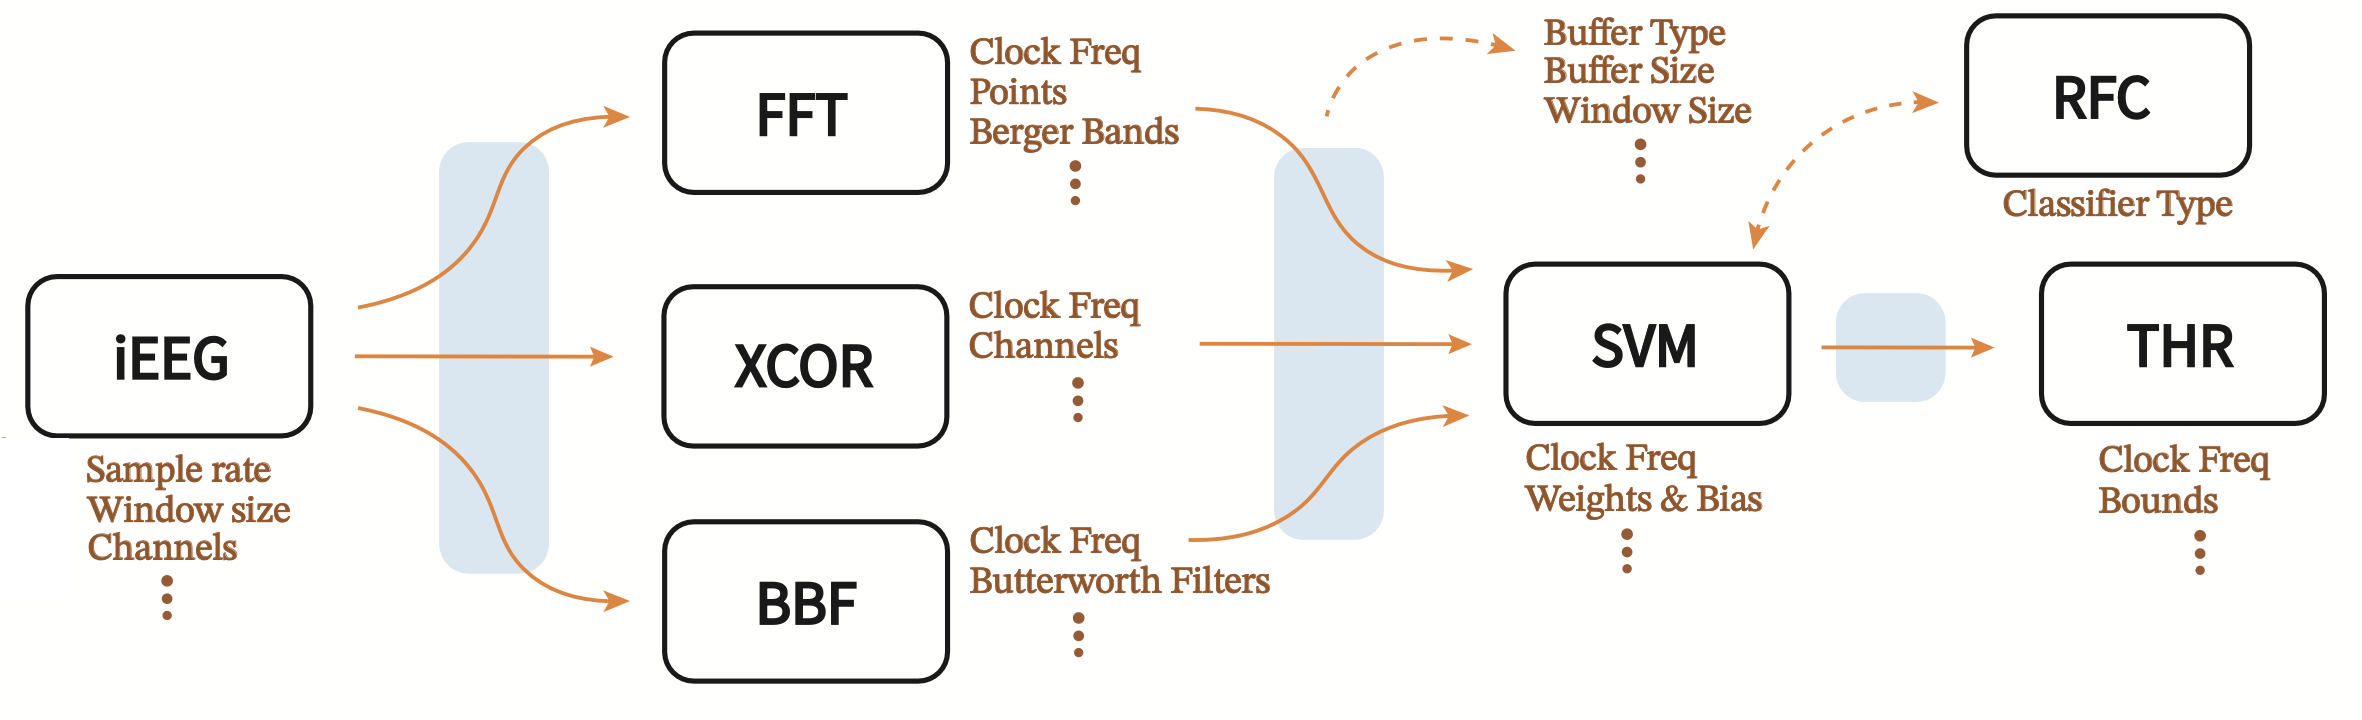
\includegraphics[width=7cm]{vis/computation_graph.png}
    \caption{Automated pipeline generation}
    \label{fig:comp_graph}
\end{figure}

\begin{figure}[htp]
    \centering
    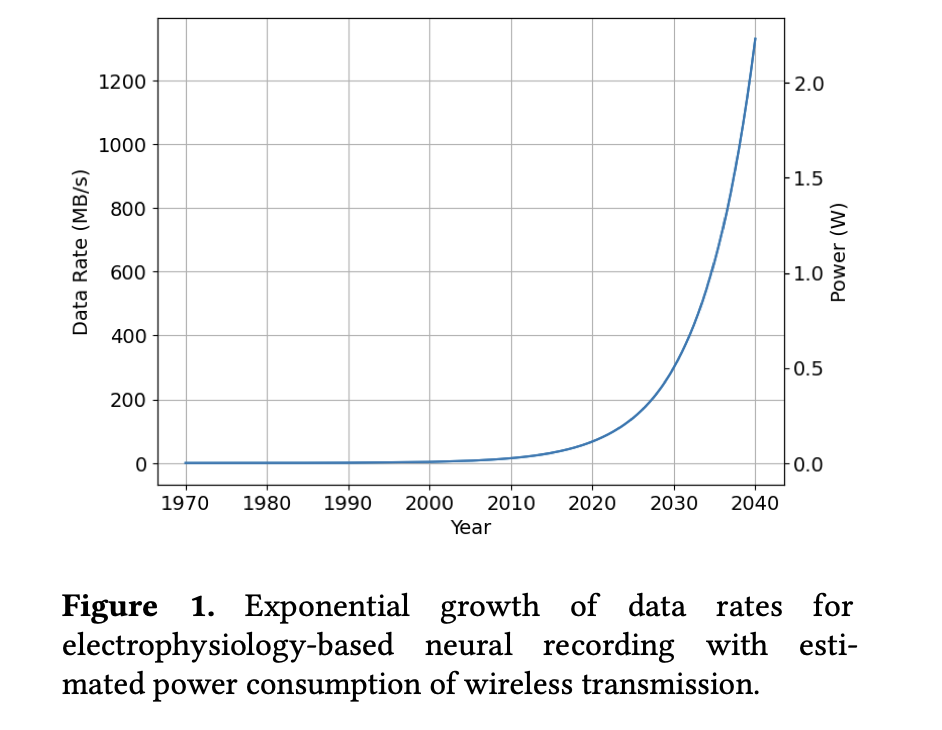
\includegraphics[width=7.5cm]{vis/neural_data_rate.png}
    \caption{Graph showing increasing neural data rates, and so the need for custom hardware based compute}
    \label{fig:comp_graph}
\end{figure}


\begin{figure}[htp]
    \centering
    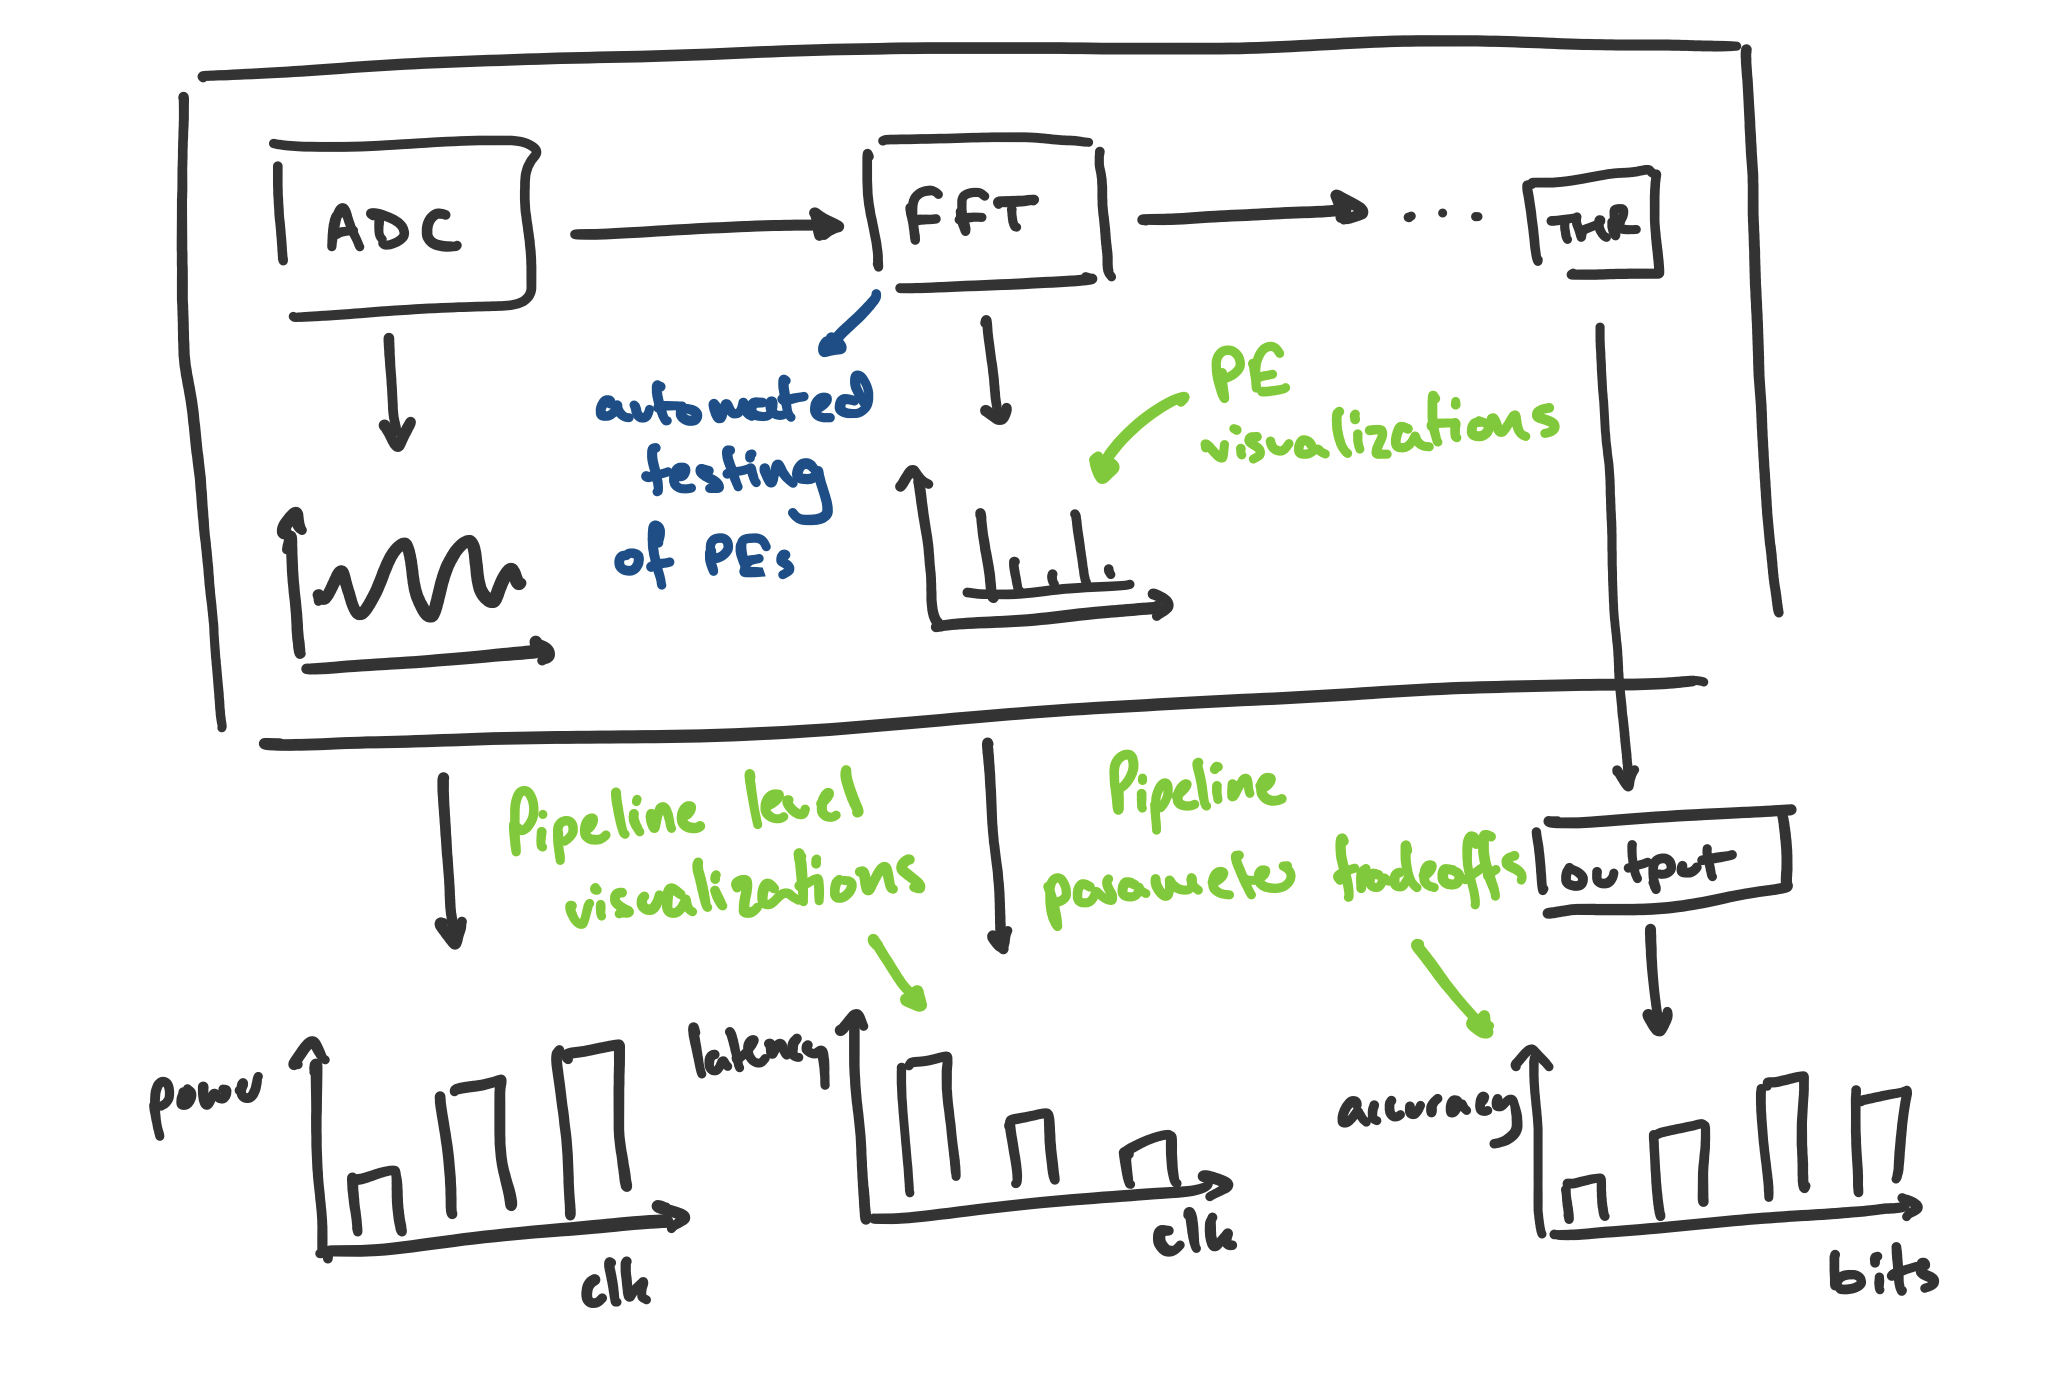
\includegraphics[width=8.25cm]{vis/vis_hierarchy.jpeg}
    \caption{Illustration showing the different visualizations at different "levels" of the pipeline}
    \label{fig:comp_graph}
\end{figure}

\begin{figure}[htp]
    \centering
    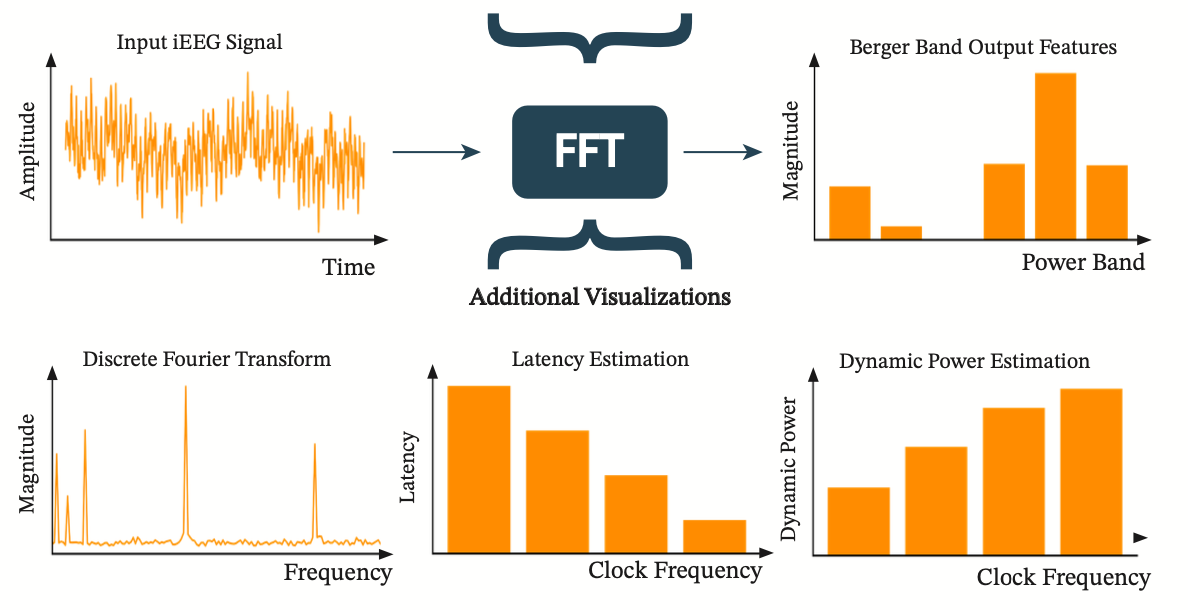
\includegraphics[width=8.25cm]{vis/PE_visualization.png}
    \caption{PE level visualizations. For NER, we want to mostly focus on algorithm validation from a hardware perspective and one or two tools (ie power estimation) to show the potential of this field.}
    \label{fig:comp_graph}
\end{figure}

\begin{figure}[htp]
    \centering
    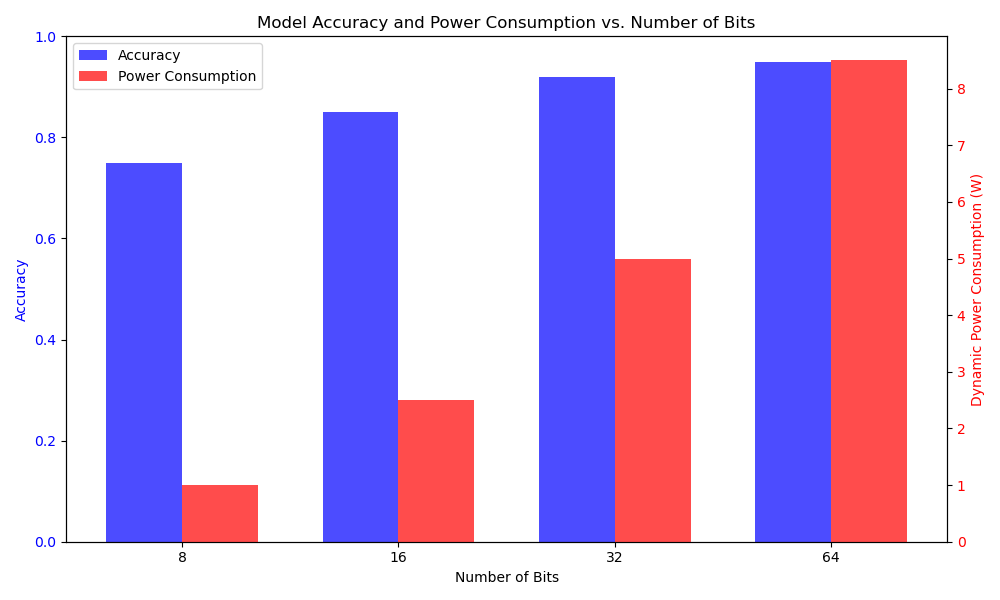
\includegraphics[width=8.25cm]{vis/Pipeline_vis.png}
    \caption{An example visualization that would be generated at the pipeline level for seeing the accuracy vs power tradeoff as data representation changes.}
    \label{fig:comp_graph}
\end{figure}

\begin{figure}[htp]
    \centering
    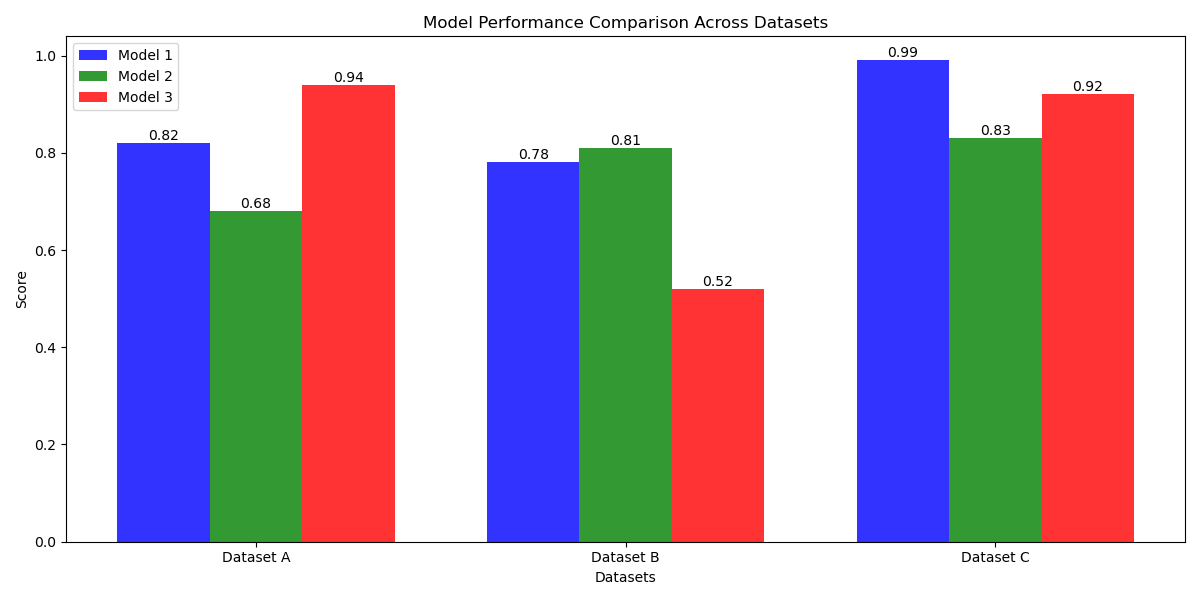
\includegraphics[width=8.25cm]{vis/Pipeline_perf.png}
    \caption{An example visualization that would be generated at the pipeline level to show the performance of different models across different datasets.}
    \label{fig:comp_graph}
\end{figure}

\section{Validation}
FPGA-based validation

Tool outputs on the x-axis, FPGA-based outputs on the y-axis. Relate the two results to one another for validation.

\section{Extrapolation}
ITRS Roadmap for technology scaling

Looking at other circuits papers for "validation", show similarity/closeness of extrapolation to existing designs in these conferences.

\section{Execution Time}
Include plots on the execution time of the tool.

\section{Other notes}

Want to keep it brief, only 4 pages for NER. Idea is to show the usefulness of the simulator specifically to neuroengineers and not go into the details of how we did things (lack of space, audience). 

The paper shown by Raghav (which was a tool accepted by NER, \href{https://drive.google.com/file/d/1-f7rhJeyTUKX2FIG0FNM0RvG3iNqYFV8/view}{link}), seems to be very simple and very specific. The bar seems to be creating a tool that can be specifically useful for neuroengineers.

Also, for tools currently thinking of power estimation and accuracy vs amt of hardware tradeoff. Thinking of making external more accurate proprietary tools (ie tools on grace) usable within our simulator for power estimation, while providing a basic solution ourselves.

The interface of gem5 is a really good way of interfacing simulators, perhaps aim to create the equivalent of gem5 for BCI hardware with "SimObject" like structure?

MATLAB conversion as well as Python.

\section{Future Work}

Making power estimation more reliable. Power estimation without Verilog. Connect the tool with an actual chip/FPGA in real-time. Automatic RTL generation from high-level code like Python.

\printbibliography

\end{document}

% next steps

% try to impress previous work section
% what the main contributions of previous ones are 
% and how you are different

% tie in the distill work (put it in similar work?)

% generalise it for computation for neuroscience
%  look at simulators for computation for neuroscience